    % \begin{frame}{Reynold's Number Range I}
    % \begin{itemize}
    %     \item Analysis of wing and tail foils at various input velocities from 30 - 60 mph. 
    %     \item Our cruise altitude (1500ft) and ground altitude (1000ft) results showed negligible difference. 
    %     \begin{figure}[htbp]
    %         \centering
    %         \begin{subfigure}{0.85\textwidth}
    %             \centering
    %             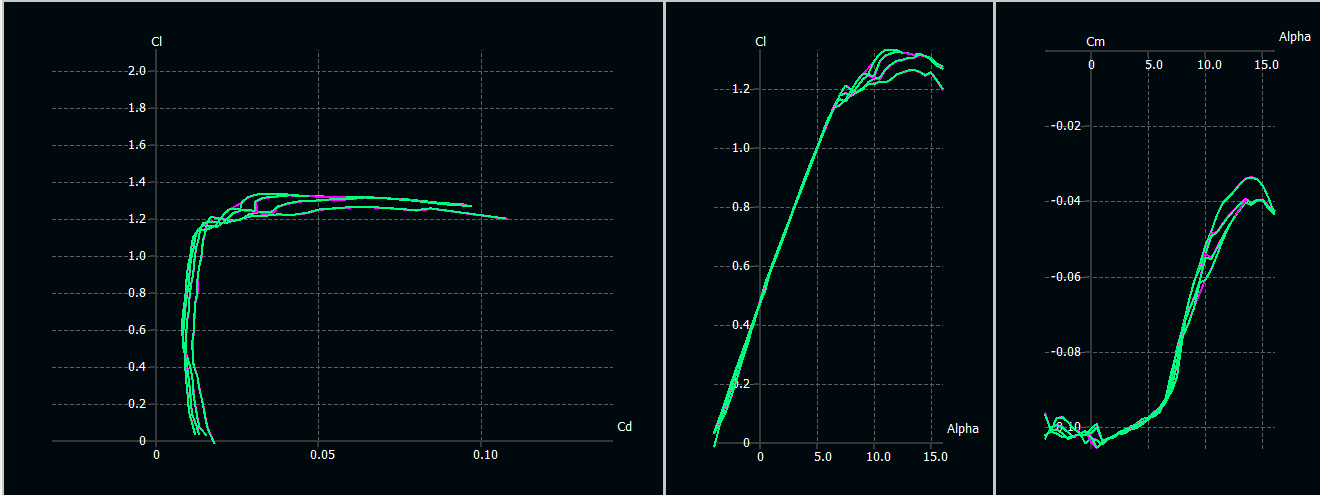
\includegraphics[width=\textwidth]{figures/groundVcruisecharts.png}
    %         \end{subfigure}
    %         \hfill
    %         \begin{subfigure}{0.4\textwidth}
    %             \centering
    %             
\includegraphics[width=\textwidth]{figures/groundVcruise_legend.png}
    %         \end{subfigure}
    % \end{figure}

    % \end{itemize}
    % \end{frame}
    % \begin{frame}{Reynold's Number Range II}
    % \begin{itemize}
    %     \item Corresponding NACA 4412 Reynold’s Range:
    %     \begin{itemize}
    %         \item 179976 to 359952 
    %     \end{itemize}
    % \end{itemize}
    %     \begin{itemize}
    %     \item Corresponding NACA 0010 Reynold’s Range:
    %     \begin{itemize}
    %         \item 134982 to 269964  
    %     \end{itemize}
    %     \item Compared to other sUAS, these Reynold's numbers were  low. This contributed to an increase in chord later in our design process.
    %     % might need a source here????????????????????????????? market researcvh????????
    % \end{itemize}
    % \end{frame}
    
% \begin{frame}{Preliminary CFD}
% \begin{itemize}
%     \item 
% \end{itemize}
% \begin{figure}[htbp]
%             \centering
% 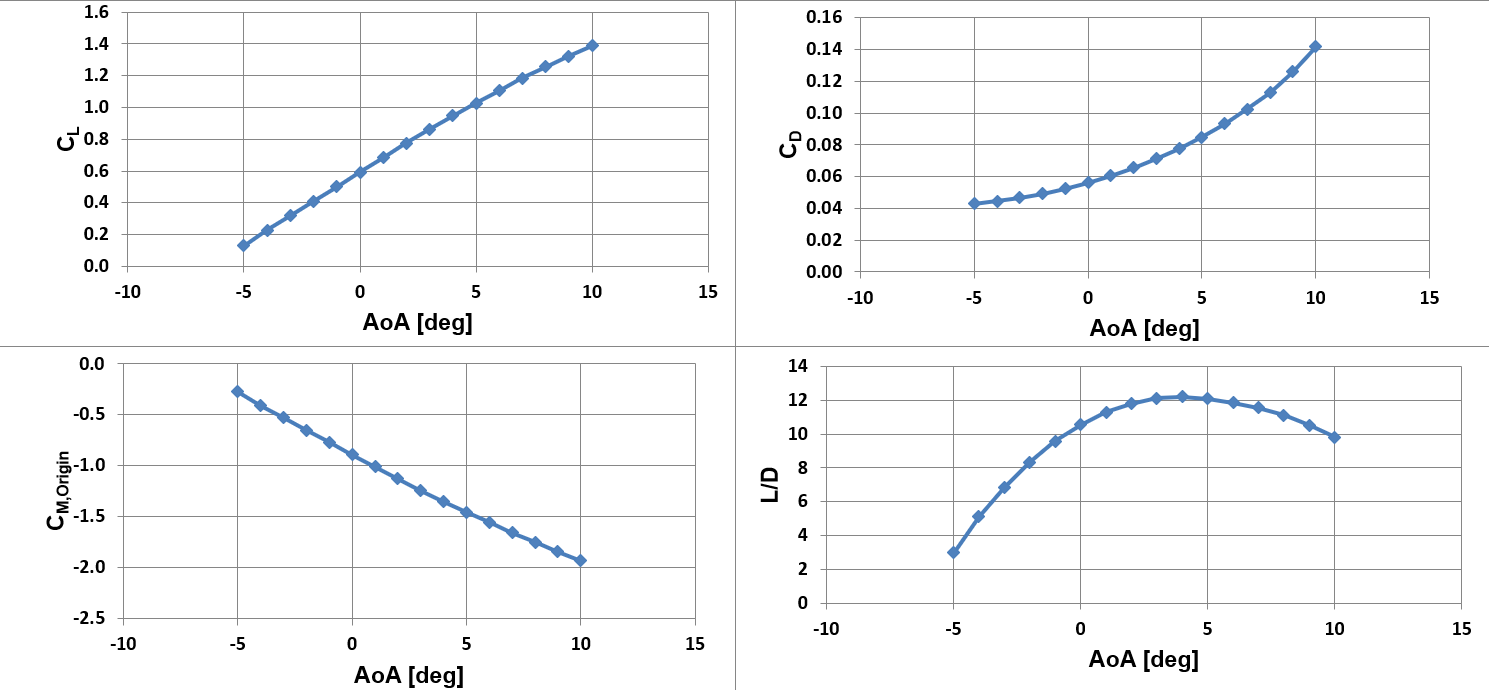
\includegraphics[width=\textwidth]{figures/prelimCFDresults.png}
% \end{figure}  
% \end{frame}
% \begin{frame}{Wing Positioning}
% put version 1.1 stuff here
% \end{frame}
% \begin{frame}{Primary Wing Airfoil Change}
%     \begin{itemize}
%         \item Due to NACA 4412 large pitching moments, the NACA 2412 was considered as a replacement
%         \item Produces less lift at same speeds than NACA 4412, but will have better pitch stability.
%     \end{itemize}
%     \centering
%          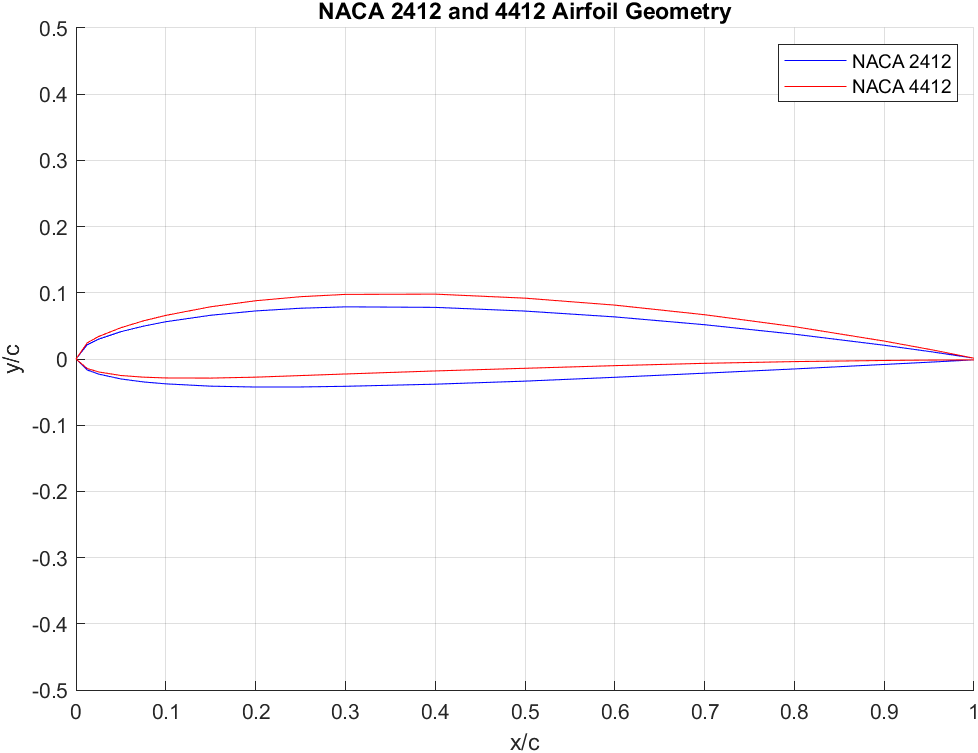
\includegraphics[width=0.7\textwidth]{figures/matlab airfoil/Figure1.png}
% \end{frame}
% \begin{frame}{Tail Wing Airfoil Change}
%     \begin{itemize}
%         \item %TALK ABOUT TAIL SELECTION WITH CORRESPONDING FIGURE
%         \item %it was copy pasted from the above section
%     \end{itemize}
%     \centering
%          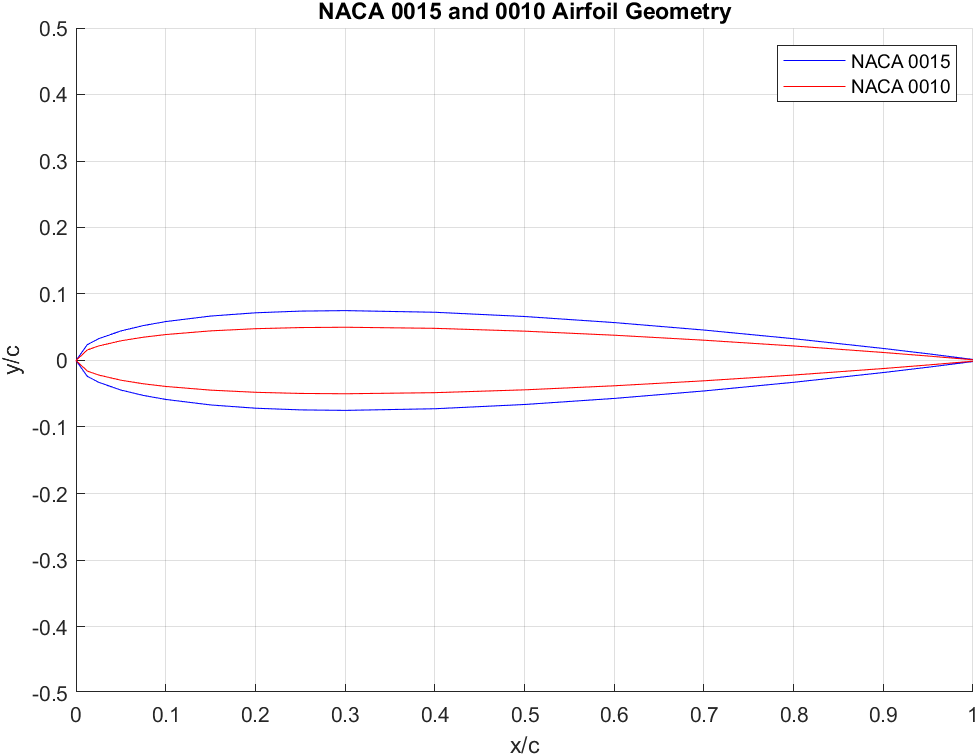
\includegraphics[width=0.7\textwidth]{figures/matlab airfoil/Figure4.png}
% \end{frame}
    
%     \begin{frame}{Version 1.0 Analysis I}
%     \begin{itemize}
%         \item Obtain preliminary CFD data of fuselage and wing to compare with previous XFLR5 data
%         \item Version 1.0 CAD drawing with dimensions in cm:
%     \end{itemize}
%     \begin{figure}[htbp]
%             \centering
%             \begin{subfigure}{1\textwidth}
%                 \centering
%                 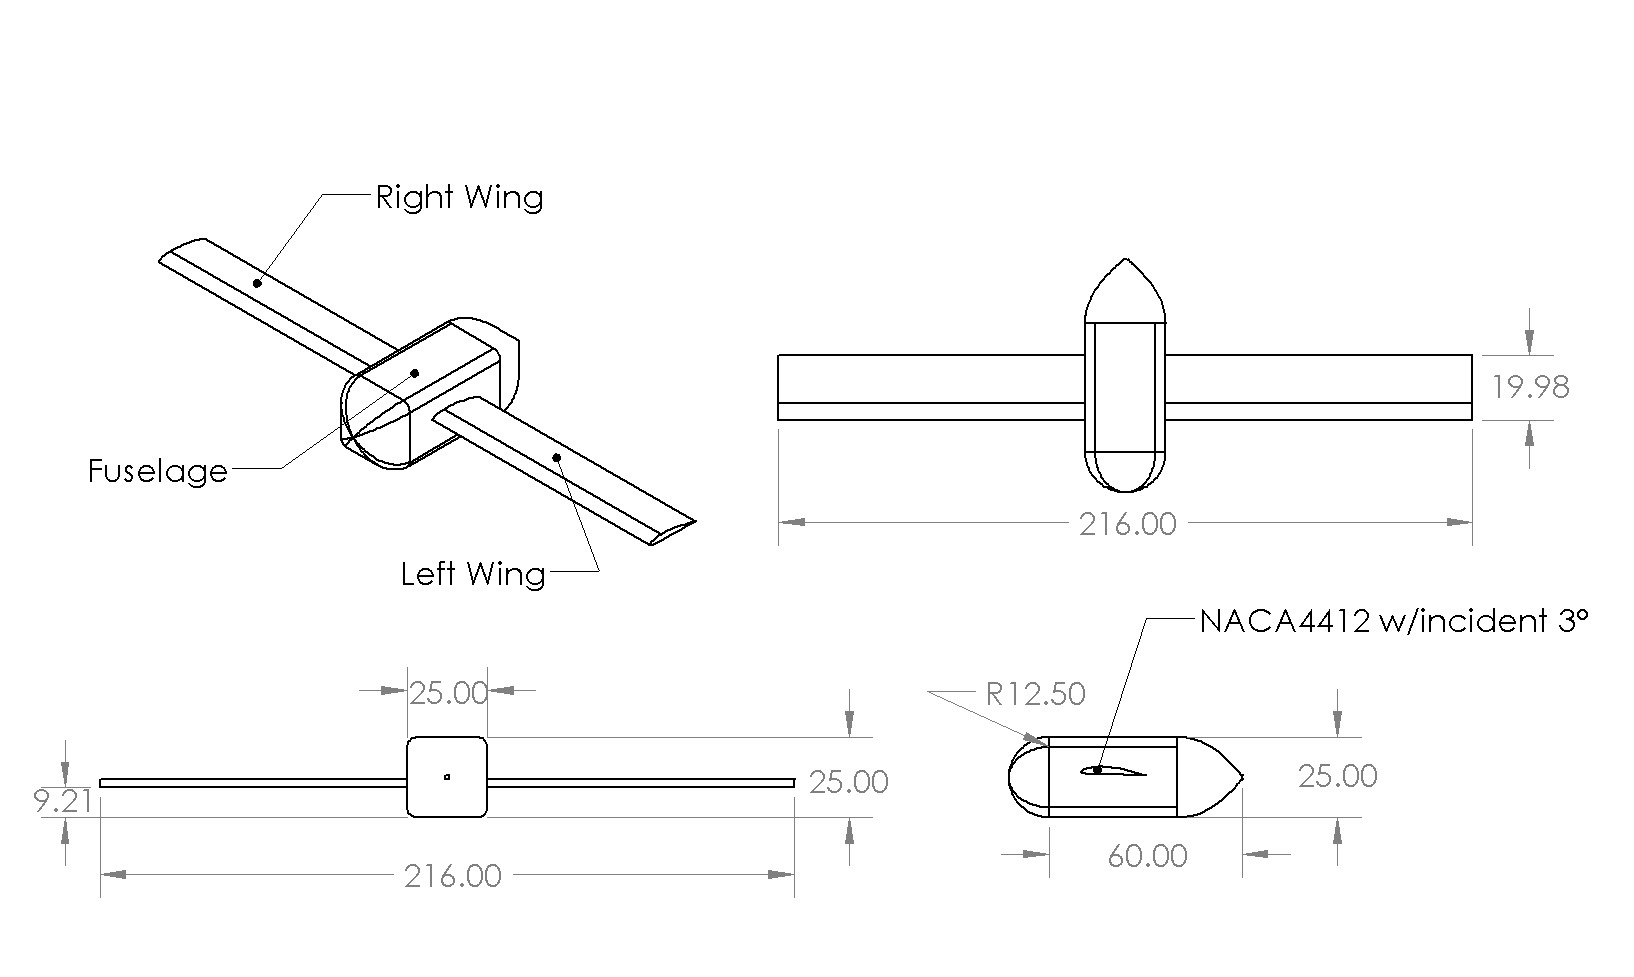
\includegraphics[width=\textwidth]{figures/FuselageAirfoilAssemDraw.png}
%             \end{subfigure}
%     \end{figure}
%     \end{frame}
    
% \begin{frame}{Version 1.0 Analysis II}
% \begin{itemize}
% \item High lift/drag ratio 
% \item Lift coefficient higher than in XFLR5 data
% %\item Wanted to change wing position and fuselage shape for next design iteration. (I don't think this is necessary? We can say it talking)
% \end{itemize}



% \end{frame}


    
%     \begin{frame}{Version 1.1 Analysis I}
%     \begin{itemize}
%  \item Analyze wing position influence on aerodynamic performance
%         \item 15 different design iterations  for different wing position 
            

%     \end{itemize}
% \begin{figure}[htbp]
%             \centering
%         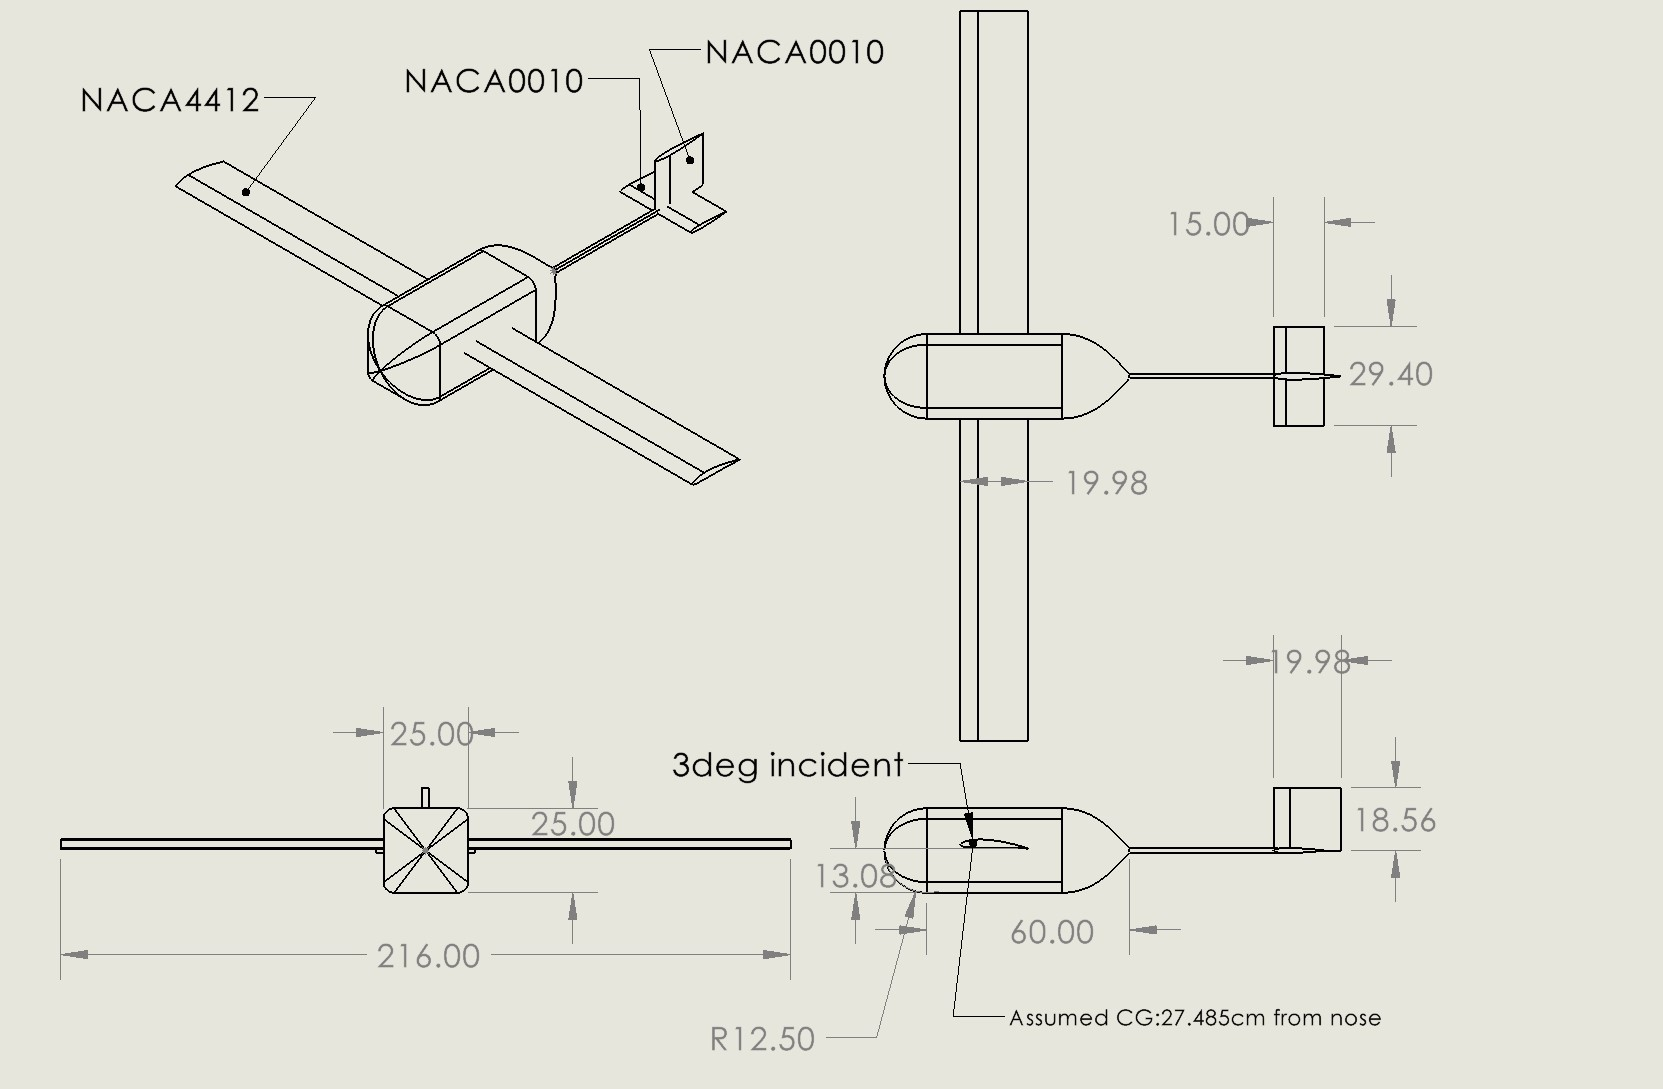
\includegraphics[width=.55\textwidth]{figures/Assem1.1.1Drawing.png}
%         \end{figure}
    
%     \end{frame}
% \begin{frame}{Version 1.1 Analysis II}
% \begin{itemize}
%     \item Most iterations had neutral points too close/too far from center of gravity (outside of static margin range). 
%     \item All iterations had pitching moments in marginally unstable regions. 
%     \item Version 1.1.12 (NACA 0015 tail and wing positioned 8 inches from nose) was chosen for 18 percent static margin and 'least-negative' pitching moment in AoA range:
% \end{itemize}
% \begin{figure}[htbp]
%             \centering
%         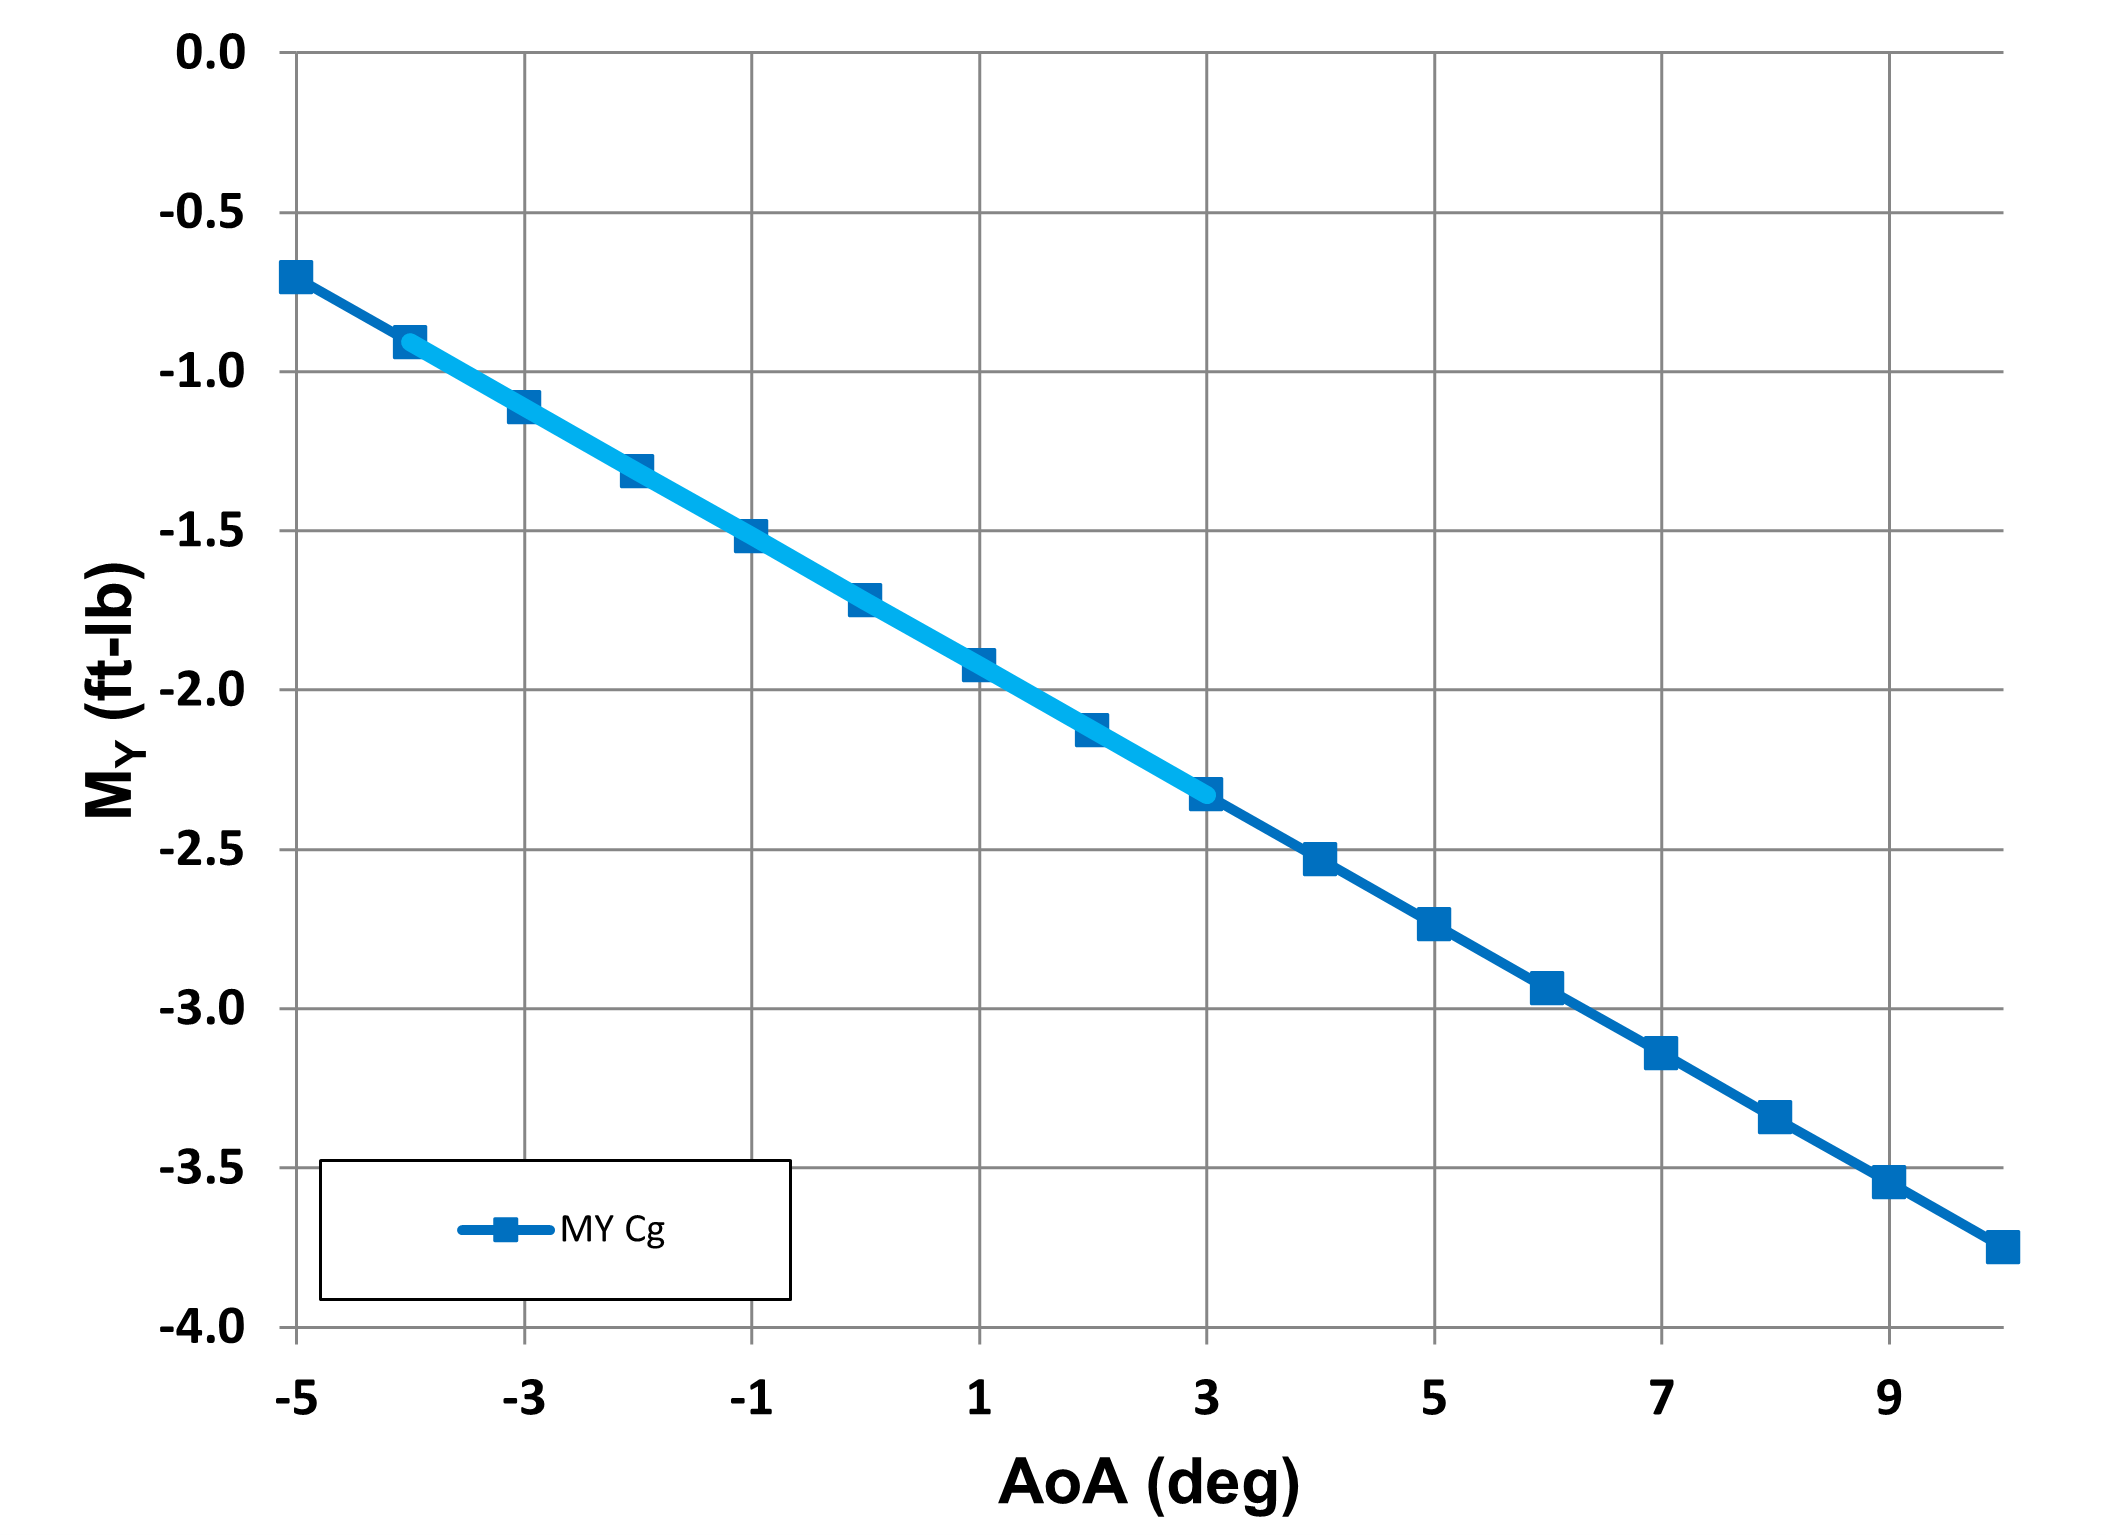
\includegraphics[width=.55\textwidth]{figures/pitchV1.1.12.png}
%         \end{figure}
% \end{frame}








% \begin{frame}{Aerodynamic Performance}
% \begin{itemize}
%     \item Evaluation of Three UAV Design Variants
%     \item Comparison of aerodynamic performance metrics to identify the optimal design
% \item Assessment based on stability, efficiency, and maneuverability for mission requirements
% \end{itemize}
% \end{frame}
% \begin{frame}{Design I}
% \begin{itemize}
%         \item \textbf{Design 1: Fixed-Wing UAV}
%         \begin{itemize}
%             %\item \includegraphics[width=0.4\textwidth]{design1_plot} % Placeholder for the plot of Design 1
%             \item Comments: Fixed-wing design optimized for endurance and longer flight times. Useful for patrolling large areas but may have limited maneuverability for close encounters.
%         \end{itemize}

%         \vspace{0.5cm} % Adjust space as needed

%         \item \textbf{Design 2: Quadrotor UAV}
%         \begin{itemize}
%             %\item \includegraphics[width=0.4\textwidth]{design2_plot} % Placeholder for the plot of Design 2
%             \item Comments: Quadrotor design offers enhanced agility and precision control, ideal for urban or densely populated event areas, but has limited range and battery life.
%         \end{itemize}

%         \vspace{0.5cm} % Adjust space as needed
% 7
%         \item \textbf{Design 3: Hybrid UAV}
%         \begin{itemize}
%            % \item \includegraphics[width=0.4\textwidth]{design3_plot} % Placeholder for the plot of Design 3
%             \item Comments: Hybrid configuration combining fixed-wing and quadrotor capabilities, aiming for a balance between endurance and maneuverability.
%         \end{itemize}
%     \end{itemize} 








% \end{frame}




% %\end{frame}

% % i moved it up :) gulp


    % \begin{frame}{Fuselage Selection}
    %     \begin{itemize}
    %         \item Three fuselage design versions evaluated 
    %         \item Selected Version 2 as the optimal design Cd0:0.0175
    %     \end{itemize}
    %     \centering
    %     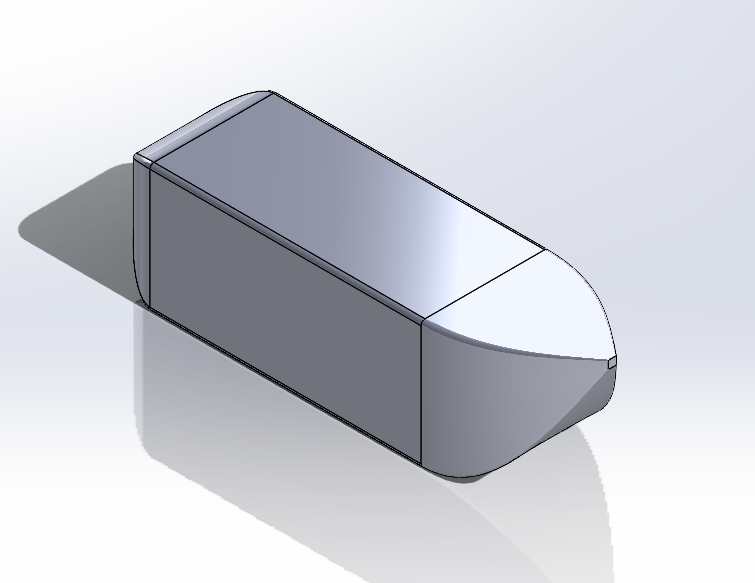
\includegraphics[width=0.6\textwidth]{fuselage1.png} 
    % \end{frame}